\documentclass[a4paper]{article}

\usepackage[utf8]{inputenc}
\usepackage[portuguese]{babel}
\usepackage{a4wide}
\usepackage[pdftex]{hyperref}
\usepackage{graphicx}
\usepackage{wrapfig}
\usepackage{amsmath}
\usepackage{caption}
\usepackage{subcaption}
\usepackage{tikz}
\usepackage{pgfplots}
\pgfplotsset{compat=1.10}
\usepgfplotslibrary{fillbetween}
\usepackage{pgfplots}
\usetikzlibrary{patterns}



\begin{document}

\begin{titlepage}
\begin{center}



\includegraphics[width=0.6\textwidth]{logo}\\[0.5cm]

{\large Universidade do Minho - Escola de Engenharia}\\[0.5cm]

{\large Relatório do trabalho prático de Desenvolvimento de Sistemas de Software}\\[0.5cm]

% Title
\rule{\linewidth}{0.5mm} \\[0.4cm]
{ \huge \bfseries Sistema de Gestão de Turnos Práticos \\[0.4cm] }
\rule{\linewidth}{0.5mm} \\[1.5cm]

% Author and supervisor
\noindent
\begin{minipage}{0.4\textwidth}
  \begin{flushleft} \large
    \emph{Autores :}\\
    Diana Costa \textsc{(A78985)}\\
    
\includegraphics[width=1.5cm]{diana}\break
    Marcos Pereira \textsc{(A79116)}\\
    
\includegraphics[width=1.5cm]{marcos}\break
    Sérgio Oliveira\textsc{(A77730)}\\
    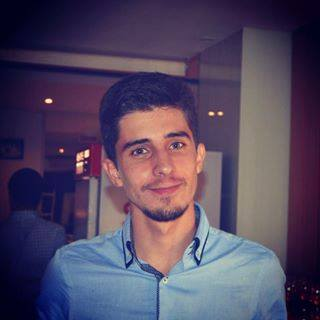
\includegraphics[width=1.5cm]{sergio}\break
    Vitor Castro\textsc{(A77870)}\\
    
\includegraphics[width=1.5cm]{vitor}\break
  \end{flushleft}
\end{minipage}%
\vfill

% Bottom of the page
{\large Versão 1.0 \\ \today}

\end{center}
\end{titlepage}




\begin{abstract}

\hspace{3mm}
\end{abstract}

\pagebreak
\tableofcontents

\pagebreak
\section{Introdução}
\label{sec:1}

\pagebreak
\section{Parte I}
\label{sec:2}

\hspace{3mm}


  

\pagebreak
\clearpage
\section{Parte II}
\label{sec:3}


\pagebreak
\section{Conclusões}
\label{sec:4}

\hspace{3mm}
\end{document}
